\newpage
\section{Architecture de la base de données}
\label{sec:bdd}

\subsection{Base de données}

Notre base de données est gérée par un système NoSQL : MongoDB. Nos données sont reparties par collections (c’est l’équivalent d’une table en SQL). Dans ces collections, les données sont écrites sous forme de document JSON. Le format JSON permet de représenter l’information de manière structurée. Un document JSON est composé de paires nom/valeurs ou de listes ordonnées de valeurs. Ces valeurs peuvent être des objets eux-mêmes représentés sous format JSON ; des tableaux ou des valeurs génériques : nombre, chaîne de caractère, booléen. 


Voilà un exemple de document que nous aurons dans la collection Revues : 


\begin{verbatimtab}[3]
{
	‘_id’ : 1,
	‘Nom’ : ‘Mai 68’,
	‘Description’ : ‘Ceci est une revue de presse sur Mai 68’,
	‘TitreArticles’ : [ 
		{ ‘idArticle’ : ‘34354’, ‘Titre’ : ‘Effervescence dans les universités françaises’ },
		{ ‘idArticle’ : ‘78e64a’,  ‘Titre’ :	‘Premières barricades de Mai 68’ }
  ]
}
\end{verbatimtab}

Chaque document dispose d’un id afin de pouvoir le retrouver rapidement. Cela permet aussi de pouvoir référencer d’autres objets de la base de données. 

Le diagramme suivant résume la modélisation de notre base de données :


\begin{figure}[H]
        \centering
        \includegraphics[width=\textwidth]{figure/ModelBDD.png}
            \caption{Modélisation de la base de données}
            \label{fig:modelbdd}
\end{figure}

Certaines informations peuvent sembler répétitives comme la liste des articles favoris qui contient les mêmes informations que celles contenues dans les documents de la collection Article. Cependant, avec MongoDB, nous ne pouvons pas faire de jointure entre les tables. Si nous voulons les informations sur l’article, il sera nécessaire de faire une deuxième requête dans la base avec l’id du document de l’article pour obtenir ces informations. C’est pourquoi certaines informations sont dupliquées, notamment celles qui seront affichées. Cela permet d'économiser une requête à la base de données et donc du temps. Pour notre exemple, lors de l’affichage de la liste des favoris dans l’espace utilisateur, il est indiqué le titre, le titre du journal, la date et un extrait de l’article. 


Chaque flèche représente une référence, c’est-à-dire que l’id du document correspondant est stockée afin de pouvoir le retrouver dans la base. Les tableaux Coord[] stockent les coordonnées du  titre ou du mot. Cela nous permettra de le mettre en surbrillance lorsqu’il est l’objet de la recherche. 

\subsection{Elasticsearch}

Elasticsearch est un moteur de recherche, il nous servira pour rechercher parmi les articles de notre base, mais aussi pour n'importe quelle requête de recherche que nous aurons besoin de faire. Elasticsearch construit un index à partir des données afin de les parcourir rapidement et de manière optimisée. Pour notre projet, Elasticsearch indexera chaque collection de la base de données.  Cela nous dispense de construire nous-mêmes l'index de la base de données et les requêtes de recherche seront plus rapides que si nous les envoyions directement à MongoDB.


Habituellement, Elasticsearch dispose de sa propre base de données qu’il indexe. Nous utilisons donc le plugin elasticsearch-river-mongodb\cite{GitRiver}. Il permet à Elasticsearch d’utiliser une base de données MongoDB comme source de données. 


De plus, à chaque ajout, mise à jour ou suppression de données dans la base MongoDB, Elasticsearch met automatiquement à jour son index. Pour cela, il est nécessaire que la base MongoDB soit en \textbf{\textit{replica set}}.  Un \textbf{\textit{replica set}} est un groupe d’instances MongoDB qui maintiennent les mêmes données. Dans ce groupe, chaque instance est accessible en lecture et il y a une instance primaire qui est la seule à être accessible en écriture. Lorsque des modifications sont faîtes dans cette instance, les modifications sont répliquées aux autres instances du groupe. Dans notre cas, la base de données MongoDB sera l’instance primaire et Elasticsearch, par le biais du plugin, sera considérée comme une instance secondaire. 

Après avoir configurer l'instance de MongoDB en \textbf{\textit{replica set}}, Elasticsearch peut créer des indexs à partir des données de MongoDB.
Pour effectuer une recherche dans la base à l’aide d’Elasticsearch, nous utiliserons utiliser l’API REST. Cette API utilise le format JSON pour les requêtes et aussi les requêtes en HTTP.


Elle est utilisée de la façon suivante :
\begin{verbatim}
http://host:port/[index]/[type]/[_action|id]
\end{verbatim}
Avec

\begin{itemize}
	\item index : Nom de l’index sur lequel porte l’opération
	\item type : Nom du type de document
	\item \_action : Nom de l’action à effectuer
	\item id : Identifiant du document
\end{itemize}


Par exemple, nous pourrons récupérer le document avec son id mais aussi effectuer une recherche d’un terme particulier :
\begin{verbatim}
http://host:port/[index]/[type]/_search?q=mai68
\end{verbatim}

Pour une recherche plus complexe, il faut envoyer une requête au format JSON :

\begin{verbatim}
{
    "query": {
        "bool": {
            "must": [
                {
                    "query_string": {
                        "default_field": "my_field",
                        "query": "text"
                    }
                }
            ],
            "must_not": [ ],
            "should": [ ]
        }
    },
    "from": 0,
    "size": 10,
    "sort": [ ]
}
\end{verbatim}

Avec
\begin{itemize}
	\item La partie \textit{must} contient les termes que doivent avoir les documents recherchés.
	\item La partie \textit{must\_not} les termes que le document ne doit pas contenir
	\item La partie \textit{should} les documents qui auront ces termes seront mis en haut de la liste
	\item \textit{from} correspond à l'indice du document par lequel vous voulez que la liste des résultats commence
	\item \textit {size} est le nombre de résultats que l'on veut récupérer
	\item \textit{sort} permet de trier les résultats
\end{itemize}
Il n'est pas nécessaire de tous les spécifier à chaque requête.


Il est aussi possible d’utiliser le plugin Head d’Elasticsearch. Il permet d’avoir accès à une interface. Depuis cette dernière, nous pouvons consulter l’état d’Elasticsearch et de ses index. Nous accédons aussi à une interface de moteur de recherche. Cependant, ce plugin nous sera moins utile car Elasticsearch sera sur un serveur, nous y accèderons donc principalement à distance.

\subsection{Communication avec php}
\subsubsection{MongoDB}

Pour communiquer avec une base MongoDB, PHP dispose d’une classe Mongo. Celle-ci permet de faire des ajouts, des modifications et des suppressions dans la base de données. 

\begin{verbatim}
$m = new MongoClient();

// select a database
$db = $m->databaseName;   
$collection = $db->databaseCollection;

$collection->insert($doc);
\end{verbatim}

Le \textit{\$doc} aura été défini avant.

\subsubsection{Elasticsearch}

Pour Elasticsearch, nous utilisons le client PHP officiel pour Elasticsearch. Ainsi, nous pouvons envoyer des requêtes à Elasticsearch et récupérer les résultats de la recherche. Ces requêtes peuvent utiliser la même syntaxe qu’une requête de l’API REST. Par exemple, dans une base de données de restaurants :

\begin{verbatimtab}
$json = '{

    "query": {
        "bool": {
            "must": [
                {
                    "query_string": {
                        "default_field": "restau.borough",
                        "query": "Bronx"
                    }
                }
            ]
        }
    }
}';

$params = [
    'index' => 'resto',
    'type' => 'restau',
    'body' => $json
];

$results = $client->search($params);
print_r($results);
\end{verbatimtab}

\newpage
Bien évidemment, Elasticsearch retourne les résultats au format JSON. Mais, le client transforme automatiquement ces données en un format lisible par PHP. La figure \ref{datajsonPhp} montre les données d'une revue au format JSON et le format que nous utiliserons avec PHP.

\begin{figure}[H]
        \centering
        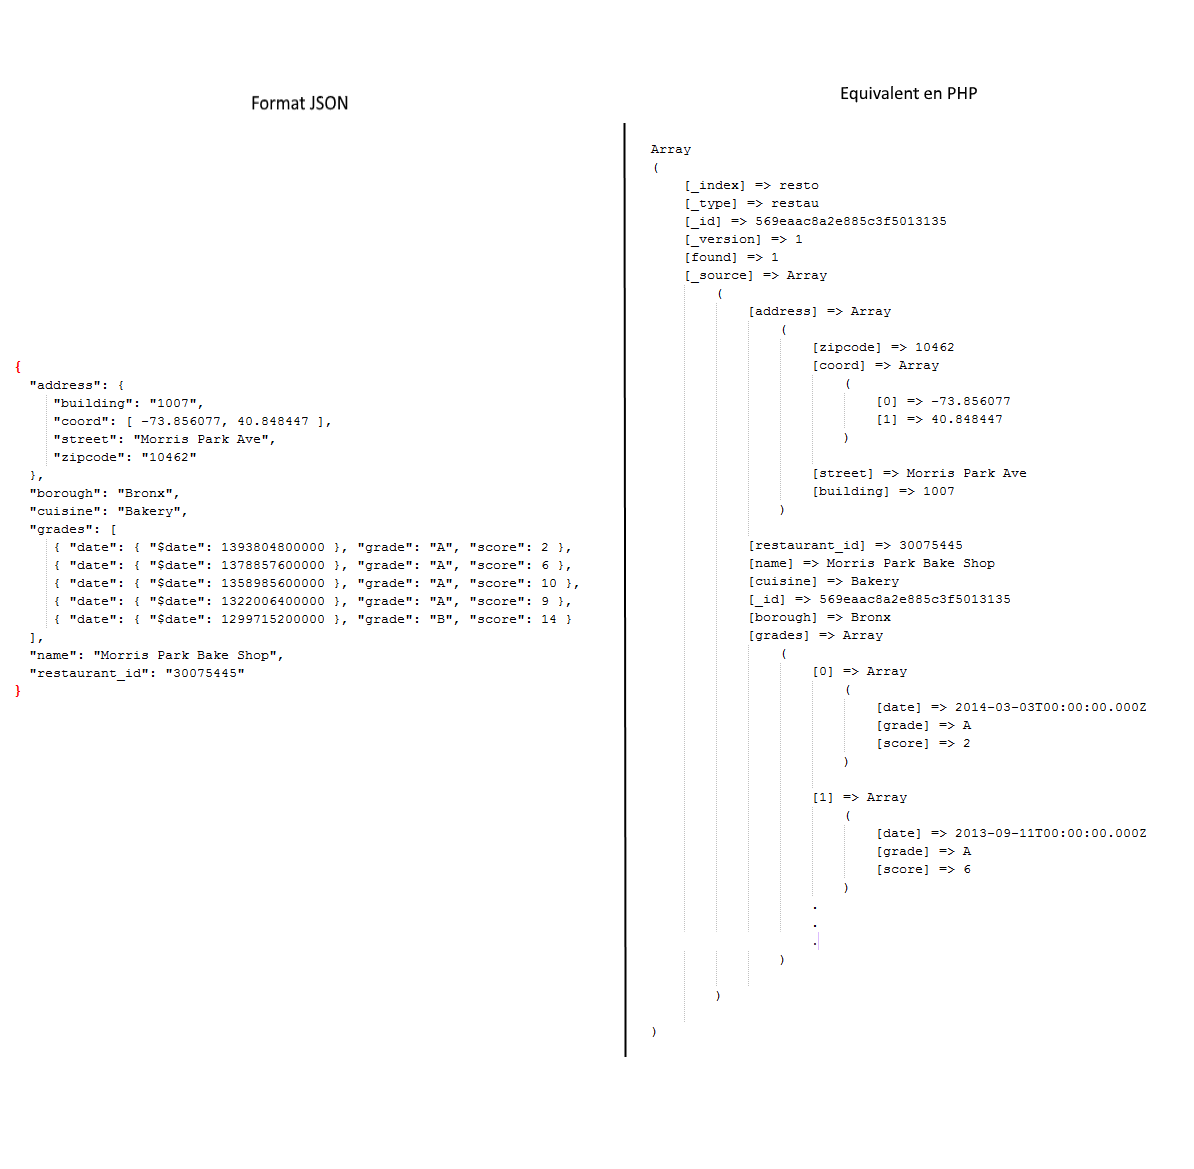
\includegraphics[width=\textwidth]{figure/dataJSONPHP.png}
            \caption{Format des données fournies par Elasticsearch}
            \label{datajsonPhp}
\end{figure}
